
\section{Càlcul numèric de derivades i integrals} \label{ap:calcul_numeric}

L'objectiu d'aquest annex és donar el fonament teòric necessari per l'anàlisi numèric de la secció \ref{sec:estudi_del_problema}.

En la resolució numèrica de problemes que involucren equacions diferencials, és necessari el càlcul de derivades i d'integrals de funcions. Atès que els ordinadors treballen amb aritmètica finita, aquests no poden fer el càlcul del límit necessari per les operacions esmentades. Per aquest motiu és necessari desenvolupar expressions per calcular aproximacions.

A continuació, es donen les nocions bàsiques pel càlcul de derivades i integrals numèriques, així com dels errors en l'aproximació. Només es demostraran el resultats rellevants.

\subsection{Interpolació polinòmica i polinomi de Taylor}

Sigui $I \subset \real$ un interval no degenerat i $f \colon I \rightarrow \real$ una funció. Es considera una xarxa de $n+1$ punts de la forma $(x_k, f(x_k))$, $k = 0 \divisionsymbol n$, amb $x_i \neq x_j$ si $i \neq j$. Per conveniència, es denota $f_k = f(x_k)$. L'objectiu és trobar un polinomi $p(x)$ tal que $p(x_k) = x_k$ per $k = 0 \divisionsymbol n$, és a dir, un polinomi que interpoli la xarxa de punts.

\begin{theorem}[Existència i unicitat del polinomi interpolador] \label{teo:existencia_unicitat}
	Existeix un únic polinomi $p_n(x)$ de grau menor o igual a $n$ que interpola la xarxa de punts. S'anomena el polinomi interpolador de $f$ en $x_0, \ldots, x_n$.
\end{theorem}

\begin{theorem}[Error en la interpolació]
	Sigui $I = [a, b] \subset \real$ un interval no degenerat i una funció $f \colon I \rightarrow \real$ de classe $\mathscr{C}^{n+1}((a,b))$. Si $x_k \in (a,b)$ per $k = 0 \divisionsymbol n$ i $p_n(x)$ és el polinomi interpolador, aleshores l'error en la interpolació és
	\[
		f(x) - p_n(x) = 
		\frac{f^{(n+1)}(\xi(x))}{(n+1)!} (x - x_0) \cdots (x - x_n)
	\]
	on $\xi(x) \in \generated{x_0, \ldots, x_n, x} \coloneqq (\min{(x_0, \ldots, x_n, x)}, \max{x_0, \ldots, x_n, x})$.
\end{theorem}

\begin{definition}
	Les diferències dividides es defineixen com
	\begin{align*}
		f[x_i] &= f(x_i) \\
		f[x_i, x_{i+1}, \ldots, x_{i+j}, x_{i+j+1}] &= 
		\frac{f[x_{i+1}, \ldots, x_{i+j+1}] - f[x_i, \ldots, x_{i+j}]}{x_{i+j+1} - x_i}
	\end{align*}
\end{definition}

\begin{prop}[Mètode de Newton]
	El polinomi interpolador de $f$ a la xarxa de punts $(x_k, f(x_k))$, $k = 0 \divisionsymbol n$ és
	\begin{align*}
		p_n(x) 
		&= \sum_{k=0}^{n} \left( f[x_0, \ldots, x_k] \prod_{j=0}^{k-1} (x - x_j) \right) \\
		&= 
		f[x_0] + 
		f[x_0, x_1] \left(x - x_0\right) + \cdots +
		f[x_0, \ldots, x_n] \left( x - x_0 \right) \cdots \left( x - x_{n-1} \right)
	\end{align*}
\end{prop}

\begin{prop}[Mètode de Lagrange]
	El polinomi interpolador de $f$ a la xarxa de punts $(x_k, f(x_k))$, $k = 0 \divisionsymbol n$ és
	\[
		p_n(x) = \sum_{k=0}^n f_k \ell_k(x)
	\]
	on $\ell_k(x)$ és el $k$-èsim polinomi de Lagrange, definit com
	\[
		\ell_k(x) = \prod_{j = 0, j \neq k}^{n} \frac{x - x_j}{x_k - x_j}
	\]
\end{prop}

Pel teorema \ref{teo:existencia_unicitat}, el polinomi interpolador és únic. Per tant, les fórmules de Newton i de Lagrange pel càlcul del polinomi interpolador són equivalents.

\begin{definition}
	El polinomi de Taylor de $f$ de grau $n$ al voltant de $x_0 \in I$ és
	\[
		P_n(x_0;x) = 
		\sum_{k=0}^n \frac{f^{(k)}(x_0)}{k!} {(x - x_0)}^k = 
		f(x_0) + f'(x_0) (x - x_0) + \cdots + 
		\frac{f^{(n)}(x_0)}{n!} (x - x_0)^n
	\]
\end{definition}

\begin{prop}[Residu de Lagrange]
	Si a més $f$ de classe $\mathscr{C}^{n+1}$ a $I$, l'error en l'aproximació de $f$ per $P_n$ és
	\[
		R_n(x_0;x) = f(x) - P_n(x_0;x) = \frac{1}{(n+1)!} f^{(n+1)}(\xi) {(x - x_0)}^{n+1}, 
		\quad \xi \in (a, b)
	\]
	és a dir,
	\[
		f(x) = 
		f(x_0) + f'(x_0) (x - x_0) + \cdots + 
		\frac{f^{(n)}(x_0)}{n!} (x - x_0)^n + 
		\frac{1}{(n+1)!} f^{(n+1)}(\xi) {(x - x_0)}^{n+1}
	\]
\end{prop}

\begin{lemma} \label{lemma:annexe_a}
	Sigui $I = [a, b]$ i $F \colon I \rightarrow \real$ contínua. Siguin $\xi_k \in I$, $\alpha_k > 0$ per $k = 1 \divisionsymbol n$. Aleshores existeix $\xi \in \tilde{I} = \generated{\xi_1, \ldots, \xi_k}$ tal que
	\[
		\sum_{k = 1}^n \alpha_k F(\xi_k) = F(\xi) \sum_{k=1}^n \alpha_k
	\]
\end{lemma}

\subsection{Càlcul numèric de derivades}

Sigui $I \subset \real$ un interval no degenerat i $f \colon I \rightarrow \real$ una funció, que es suposarà tant regular com calgui. Donat $a \in \real$, es vol calcular $f'(a)$. Es construirà el polinomi interpolador $p_m(x)$ en els punts $(x_0, f_0), \ldots, (x_m, f_m)$ i s'aproximarà $f'(a) \approx p_m'(a)$.

\subsubsection*{Diferència finita endavant}

Si $m = 1$, es prenen els punts $x_0 = a$ i $x_1 = a + h$, amb $h > 0$. El polinomi interpolador és $p_1(x) = f[x_0] + f[x_0,x_1](x - x_0)$ i l'aproximació de la derivada és 
\[
	f'(a) \approx 
	p_1'(a) = 
	f[x_0,x_1] = 
	\frac{f(x_1) - f(x_0)}{x_1 - x_0} = 
	\frac{f(a + h) - f(a)}{h}
\]
L'error comés es troba a partir de la fórmula de Lagrange,
\[
	f(a+h) = f(a) + f'(a) h + \frac{f''(\xi)}{2} h^2 \Longrightarrow
	f'(a) = \frac{f(a+h) - f(a)}{h} - \frac{f''(\xi)}{2} h
\]
Per tant l'error és $-\frac{f''(\xi)}{2} h$. Es diu que la diferència finita endavant és una aproximació de primer ordre.

\subsubsection*{Diferència finita endarrere}

Si $m = 1$, es prenen els punts $x_0 = a - h$ i $x_1 = a$, amb $h > 0$. El polinomi interpolador és $p_1(x) = f[x_0] + f[x_0,x_1](x - x_0)$ i l'aproximació de la derivada és 
\[
	f'(a) \approx 
	p_1'(a) = 
	f[x_0,x_1] = 
	\frac{f(x_1) - f(x_0)}{x_1 - x_0} = 
	\frac{f(a) - f(a-h)}{h}
\]
L'error és $\frac{f''(\xi)}{2} h$, i és novament una aproximació de primer ordre.

\subsubsection*{Diferència finita centrada}

Si $m = 2$, es prenen els punts $x_0 = a - h$, $x_1 = a$ i $x_2 = a + h$, amb $h > 0$. El polinomi interpolador és
\[
	p_2(x) = f[x_0] + f[x_0,x_1] (x - x_0) + f[x_0,x_1,x_2] (x - x_0) (x - x_1)
\]
i l'aproximació de la derivada
\begin{align*}
	f'(x) &\approx p_2'(x) = f[x_0,x_1] + f[x_0,x_1,x_2] (2 x - (x_0 + x_1)) \\
	f'(a) &\approx p_2'(a) = f[x_0,x_1] = \frac{f(a + h) - f(a - h)}{2 h}
\end{align*}
Trobem l'error comés. Calculem el polinomi de Taylor de $f$ al voltant de $a$ com segueix:
\begin{align*}
	f(a + h) &= f(a) + f'(a) h + \frac{f''(a)}{2!} h^2 + \frac{f'''(\xi_1)}{3!} h^3, 
	\quad \xi_1 \in (a, a + h) \\
	f(a - h) &= f(a) - f'(a) h + \frac{f''(a)}{2!} h^2 - \frac{f'''(\xi_2)}{3!} h^3, 
	\quad \xi_2 \in (a-h, a)
\end{align*}
Restant i dividint per $2 h$,
\[
	\frac{f(a + h) - f(a - h)}{2 h} = f'(a) + \frac{f'''(\xi_1) + f'''(\xi_2)}{2 \cdot 3!} h^2
\]
Pel lema \ref{lemma:annexe_a}, existeix $\xi \in \generated{\xi_1, \xi_2}$ tal que
\[
	\frac{f(a + h) - f(a - h)}{2 h} = f'(a) + \frac{f'''(\xi)}{3!} h^2
\]
Així la diferència finita centrada és una aproximació de segon ordre.

\subsection{Càlcul numèric d'integrals} 


Sigui $I = [a, b] \subset \real$ un interval no degenerat i $f \colon I \rightarrow \real$ una funció contínua. Volem calcular la integral $\int_a^b f(x) \dd{x}$. Prendrem $m + 1$ abscisses $a \leq x_0 < x_1 < \ldots < x_m \leq b$ en $[a,b]$, típicament equiespaiades. Construirem el polinomi interpolador $p_m(x)$ de $f$ en la xarxa $(x_k,f_k)$, $k = 0 \divisionsymbol m$ i calcularem la integral com
\[
	\int_a^b f(x) \dd{x} \approx 
	\int_a^b p_m(x) \dd{x} = 
	\int_a^b \sum_{k=0}^m f_k \ell_k(x) = 
	\sum_{k=0}^m f_k \underbrace{\int_a^b \ell_k(x) \dd{x}}_{W_k} = 
	\sum_{k=0}^m f_k W_k 
\]
Les constants $W_0, \ldots, W_m$ reben el nom de pesos de la fórmula d'integració.

\subsubsection*{Fórmula del rectangle}

Si $m = 0$, prenem $x_0 = \frac{a + b}{2}$. El polinomi interpolador és $p_0(x) = f[x_0] = f\left(\frac{a + b}{2}\right)$. Aproximem la integral com
\[
	\int_a^b f(x) \dd{x} \approx \int_a^b p_0(x) \dd{x} = (b - a) f\left(\frac{a + b}{2}\right)
\]
A la figura \ref{fig:formula_rectangle} es representa la interpretació geomètrica de la integral i l'aproximació.

\begin{figure}[h]
	\centering
	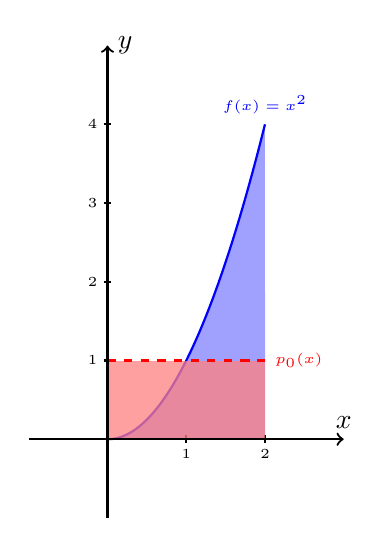
\begin{tikzpicture}[darkstyle/.style={circle,draw,fill=white}]
		\fill[blue!50!white, domain=0:2, variable=\x, opacity=0.75] (0, 0) -- plot ({\x}, {\x*\x}) -- (2, 0) -- cycle;
		\draw[scale=1, domain=0:2, smooth, variable=\x, blue, thick] plot (\x, {\x*\x}) node[above]{\tiny{$f(x) = x^2$}};		
		\foreach \t in {1,2}
			\draw[black, thick] (\t, 0.05) -- node[anchor=north]{\tiny{\t}} (\t, -0.05);
		\foreach \t in {1,...,4}
			\draw[black, thick] (-0.05, \t) -- node[anchor=east]{\tiny{\t}} (0.05, \t);
			
		\fill[red!50!white, opacity=0.75] (0, 0) rectangle (2,1);
		\draw[scale=1, domain=0:2, smooth, variable=\x, red, thick, dashed] plot (\x, 1) node[right]{\tiny{$p_0(x)$}};		
		\draw[->, thick] (-1, 0) -- (3, 0) node[above] {$x$};
		\draw[->, thick] (0, -1) -- (0, 5) node[right] {$y$};
	\end{tikzpicture}
	\caption{Fórmula del rectangle.}
	\label{fig:formula_rectangle}
\end{figure}

\begin{prop}
	Sigui $h = b - a > 0$ i $f \in \mathscr{C}^2([a,b])$. L'error comés en la fórmula del rectangle és
	\[
		E = \int_a^b f(x) \dd{x} - h f\left(\frac{a + b}{2}\right) = \frac{h^3}{24} f''(\eta),
		\quad 
		\eta \in (a, b)
	\]
\end{prop}
\begin{proof}
	Sigui $c = \frac{a + b}{2}$, llavors el polinomi de Taylor al voltant de $c$ fins ordre 2 és,
	\[
		f(x) = f(x) + \frac{f'(c)}{2!} (x - c) + \frac{f''(\sigma(x))}{2!} (x - c)^2, \quad 
		\sigma(x) \in \generated{x, c}
	\]
	Aleshores
	\[
		E = 
		\int_a^b \left( f(x) - p_0(x) \right) \dd{x} = 
		\int_a^b f'(c) (x - c) \dd{x} + \int_a^b \frac{f''(\sigma(x))}{2!} (x - c)^2 \dd{x} = 
		\cdots = 
		\frac{f''(\eta)}{24} h^3
	\]
\end{proof}

\subsubsection*{Fórmula del trapezi}

Si $m = 1$, es prenen $x_0 = a$, $x_1 = b$ i $h = b - a > 0$. Aleshores
\[
	p_1(x) = 
	\sum_{k=0}^2 f_k \ell_k(x) = 
	f(a) \frac{x - b}{a - b} + 
	f(b) \frac{x - a}{b - a}
\]
Es calculen els pesos de la fórmula:
\begin{align*}
	W_0 &= 
	\int_a^b \ell_0(x) \dd{x} = 
	\int_a^b \frac{x - b}{a - b} \dd{x} = 
	\cdots =
	\frac{h}{2} \\
	W_1 &= 
	\int_a^b \ell_1(x) \dd{x} = 
	\int_a^b \frac{x - a}{b - a} \dd{x} = 
	\cdots =
	\frac{h}{2} 
\end{align*}
D'aquesta manera, la fórmula d'integració queda
\[
	\int_a^b f(x) \dd{x} \approx
	\sum_{k=0}^1 f_k W_k = \frac{f(a) + f(b)}{2} h
\]

En la figura \ref{fig:formula_trapezi} es mostra la interpretació geomètrica de la fórmula del trapezi.

\begin{figure}[h]
	\centering
	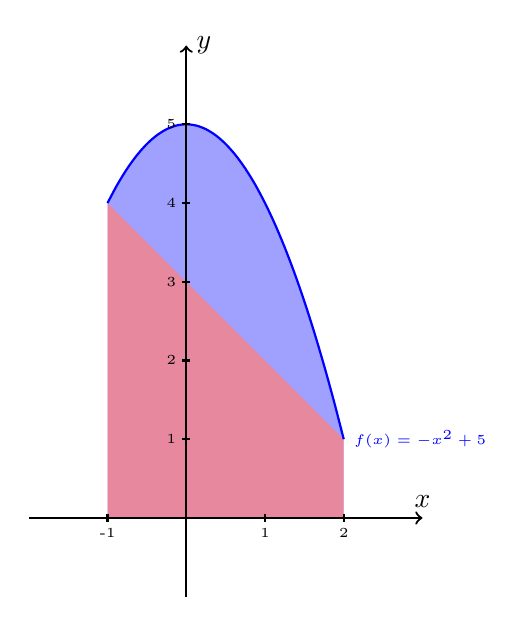
\begin{tikzpicture}[darkstyle/.style={circle,draw,fill=white}]
		\fill[blue!50!white, domain=-1:2, variable=\x, opacity=0.75] (-1, 4) -- plot ({\x}, {-\x*\x+5}) -- (2, 0) -- (-1,0) -- cycle;
%		\draw[scale=1, domain=-1:2, smooth, variable=\x, blue, thick] plot (\x, {\x*\x+1}) node[above]{\tiny{$f(x) = x^2$}};		
		
		\fill[red!50!white, opacity=0.75] (-1, 4) -- (2,1) -- (2,0) -- (-1,0) -- cycle;
		
		\draw[scale=1, domain=-1:2, smooth, variable=\x, blue, thick] plot ({\x}, {-\x*\x+5}) node[anchor=west]{\tiny{$f(x) = -x^2+5$}};		
		
		\draw[->, thick] (-2, 0) -- (3, 0) node[above] {$x$};
		\draw[->, thick] (0, -1) -- (0, 6) node[right] {$y$};
		
		
		\foreach \t in {-1}
			\draw[black, thick] (\t, 0.05) -- node[anchor=north]{\tiny{\t}} (\t, -0.05);
		\foreach \t in {1,2}
		\draw[black, thick] (\t, 0.05) -- node[anchor=north]{\tiny{\t}} (\t, -0.05);
		\foreach \t in {1,...,5}
		\draw[black, thick] (-0.05, \t) -- node[anchor=east]{\tiny{\t}} (0.05, \t);
		
	\end{tikzpicture}
	\caption{Fórmula del trapezi.}
	\label{fig:formula_trapezi}
\end{figure}

\noindent
A continuació, es prova que la fórmula del trapezi dona una aproximació de tercer ordre pel càlcul de la integral.

\begin{prop}
	Sigui $I = [a, b] \in \real$ i $f \in \mathscr{C}^2(I)$. L'error comés en la fórmula del trapezi és
	\[
		E = \int_a^b f(x) \dd{x} - \frac{f(a) + f(b)}{2} h = -\frac{f''(c)}{12} h^3, \quad
		c \in (a, b)
	\]
\end{prop}
\begin{proof}
	Es considera el canvi de variable $x = a + h t$, $\dd{x} = h \dd{t}$. S'aprofita la fórmula de l'error en la interpolació polinòmica
	\begin{align*}
		E = 
		\int_a^b \left(f(x) - p_1(x) \right) \dd{x} = 
		\int_a^b \frac{f''(\xi)}{2!} (x - a)(x - b) \dd{x} = 
		\frac{f''(c)}{2} \int_a^b (x - a)(x - b) \dd{x} = 
		-\frac{h^3}{12} f''(c)
	\end{align*}
\end{proof}